\documentclass[]{beamer}
\usepackage{graphicx} % For including single page pdfs
\usepackage{bm}       % bold math
\usepackage{pgffor}   % for loop
\usepackage{tikz}
\usepackage{multimedia}
\usepackage{layouts}
\usepackage{hyperref}



\newcommand{\lik}{\mathcal{L}}
\newcommand{\posterior}{\mathcal{P}}
\newcommand{\prior}{\pi}
\newcommand{\ev}{\mathcal{Z}}

\newcommand{\prob}{\mathrm{P}}

\newcommand{\PR}{\mathcal{P}_\mathcal{R}}
\newcommand{\Pknotj}[1]{\mathcal{P}_{#1}}
\newcommand{\Nknots}{N_\mathrm{knots}}
\newcommand{\nlive}{n_\mathrm{live}}

\newcommand{\movablecross}[1]{%
  \draw[->](#1) -- ++(0:\croslen);
  \draw[->](#1) -- ++(90:\croslen);
  \draw[->](#1) -- ++(180:\croslen);
  \draw[->](#1) -- ++(270:\croslen);
  \fill[red!70!black] (#1) circle (2pt);
}

\newcommand{\movablevert}[1]{%
  \draw[->](#1) -- ++(90:\croslen);
  \draw[->](#1) -- ++(270:\croslen);
  \fill[red!70!black] (#1) circle (2pt);
}





\setbeamertemplate{navigation symbols}{} % Turn off that bottom bar


\title{PolyChord \& the future of nested sampling}
\subtitle{Tools for sampling, Parameter Estimation and Bayesian Model Comparison}
\author[Handley] % (optional, for multiple authors)
{Will Handley\\ \small{wh260@cam.ac.uk}}
\institute[University of Cambridge] % (optional)
{%
Supervisors: Anthony Lasenby \& Mike Hobson \\
Astrophysics Group \\
Cavendish Laboratory \\
University of Cambridge
}
\date{Monday 9\textsuperscript{th} May, 2016}



\begin{document}

\begin{frame}
  \titlepage
\end{frame}

\begin{frame}
  \tableofcontents
\end{frame}


\section{Parameter estimation \& model comparison}
%\begin{frame}
%  \frametitle{Notation} 
%
%  \begin{itemize}
%      \pause
%    \item Data: $D$
%      \pause
%    \item Model: $M$
%      \pause
%    \item Parameters: $\Theta$
%      \pause
%    \item Likelihood: $\prob(D|\Theta,M)=\lik(\Theta)$
%      \pause
%    \item Posterior: $\prob(\Theta|D,M)=\posterior(\Theta)$
%      \pause
%    \item Prior: $\prob(\Theta|M)=\prior(\Theta)$
%      \pause
%    \item Evidence: $\prob(D|M)=\ev$
%  \end{itemize}
%
%
%\end{frame}

\begin{frame}
  \frametitle{What is nested sampling?}
  \begin{itemize}
    \pause\item Nested sampling is an alternative sampling approach. 
    \pause\item Unlike traditional methods, it does not sample from the posterior directly.
    \pause\item Instead it gradually compresses the prior onto the posterior.
    \pause\item In doing so, it circumvents many issues (dimensionality, topology, geometry) that beset normal approaches.
    \pause\item Similar to simulated annealing, but automatically picks the ``correct'' annealing schedule.
  \end{itemize}
\end{frame}

\begin{frame}
  \frametitle{Bayes' theorem}
  \framesubtitle{Parameter estimation}

  \pause
  What does data tell us about the params $\Theta$ of our model $M$?
    \[\prob(\Theta|D,M) = \frac{\prob(D|\Theta,M) \prob(\Theta|M) }{ \prob(D|M) }\] 
    \pause
    \[\text{Posterior } = \frac{\text{Likelihood} \times \text{Prior} } {\text{Evidence} }\] 
    \pause
    \[ \posterior(\Theta)= \frac{\lik(\Theta) \prior(\Theta)} {\ev}\] 

\end{frame}

\begin{frame}
  \frametitle{Bayes' theorem}
  \framesubtitle{Model comparison}
  \pause
  What does data tell us about our model $M_i$?
  \pause
    \[\prob(M_i|D) = \frac{\prob(D|M_i) \prob(M_i) }{ \prob(D) }\] 

  \pause
    \[\prob(M_i|D) = \frac{\ev_i \: \mu_i}{\sum_k \ev_k \: \mu_k}\] 

  \pause
  Model averaging:
  \begin{itemize}
        \item Multiple models with posterior on the same parameter: ${\prob(y|M_i,D)}$
  \end{itemize}
  \[\prob(y|D) = \sum_i \prob(y|M_i,D) \prob(M_i|D)\]


\end{frame}

%\begin{frame}
%  \frametitle{Parameter estimation \& model comparison} 
%  \framesubtitle{The challenge}
%
%  \pause
%  Both of these are challenging things to compute.
%  \begin{itemize}
%      \pause
%    \item Markov-Chain Monte-Carlo (MCMC) can solve the first of these (kind of)
%      \pause
%    \item Nested sampling (NS) promises to solve both simultaneously.
%  \end{itemize}
% 
%\end{frame}
%
%\begin{frame}
%  \frametitle{Parameter estimation \& model comparison} 
%  \framesubtitle{Why is it difficult?} 
%
%	\begin{columns}
%	\begin{column}{0.5\textwidth}
%		\begin{enumerate}
%          \pause\item In high dimensions, posterior $\posterior$ occupies a vanishingly small region of the prior $\prior$.
%          \pause\item Worse, you don't know where this region is.
%		\end{enumerate}
%	\end{column}
%	\begin{column}{0.5\textwidth}
%		\includegraphics<1->[width=\textwidth]{figures/posteriors}	
%	\end{column}
%	\end{columns}
%    \begin{itemize}
%      \pause\item Describing an $N$-dimensional posterior fully is impossible.
%      \pause\item {\em Sampling\/} the posterior is an excellent compression scheme.
%    \end{itemize}
% 
%\end{frame}


\section{Metropolis Hastings}

\begin{frame}
  \frametitle{Markov-Chain Monte-Carlo (MCMC)} 
  \framesubtitle{Metropolis-Hastings, Gibbs, Hamiltonian\ldots} 
  \begin{itemize}
      \pause
    \item Turn the $N$-dimensional problem into a one-dimensional one.
      \pause
    \item Explore the space via a biased random walk.
      \begin{enumerate}
          \pause
        \item Pick random direction
          \pause
        \item Choose step length
          \pause
        \item If uphill, make step\ldots
          \pause
        \item \ldots otherwise sometimes make step. 
      \end{enumerate}
  \end{itemize}
 
\end{frame}

\begin{frame}
  \frametitle{MCMC in action} 
  \movie[width=\textwidth,height=0.52\textwidth]{%
  \includegraphics[width=\textwidth]{movies/MCMC_0.pdf}}{movies/MCMC.mp4}
\end{frame}
\begin{frame}
  \frametitle{MCMC in action} 
  \includegraphics[width=\textwidth]{movies/MCMC_1.pdf}
\end{frame}

\begin{frame}
  \frametitle{When MCMC fails} 
  \framesubtitle{Burn in} 
  \movie[width=\textwidth,height=0.52\textwidth]{%
  \includegraphics[width=\textwidth]{movies/MCMC_burn_in_0.pdf}}{movies/MCMC_burn_in.mp4}
\end{frame}
\begin{frame}
  \frametitle{When MCMC fails} 
  \framesubtitle{Burn in} 
  \includegraphics[width=\textwidth]{movies/MCMC_burn_in_1.pdf}
\end{frame}

\begin{frame}
  \frametitle{When MCMC fails} 
  \framesubtitle{Tuning the proposal distribution} 
  \movie[width=\textwidth,height=0.52\textwidth]{%
  \includegraphics[width=\textwidth]{movies/MCMC_proposal_0.pdf}}{movies/MCMC_proposal.mp4}
\end{frame}
\begin{frame}
  \frametitle{When MCMC fails} 
  \framesubtitle{Tuning the proposal distribution} 
  \includegraphics[width=\textwidth]{movies/MCMC_proposal_1.pdf}
\end{frame}

\begin{frame}
  \frametitle{When MCMC fails} 
  \framesubtitle{Multimodality} 
  \movie[width=\textwidth,height=0.52\textwidth]{%
  \includegraphics[width=\textwidth]{movies/MCMC_multimodal_0.pdf}}{movies/MCMC_multimodal.mp4}
\end{frame}
\begin{frame}
  \frametitle{When MCMC fails} 
  \framesubtitle{Multimodality} 
  \includegraphics[width=\textwidth]{movies/MCMC_multimodal_1.pdf}
\end{frame}

\begin{frame}
  \frametitle{When MCMC fails} 
  \framesubtitle{Phase transitions} 

  \includegraphics[width=\textwidth]{figures/phase_transition}
 
\end{frame}

\begin{frame}
  \frametitle{When MCMC fails} 
  \framesubtitle{The real reason\ldots} 

  \begin{itemize}
    \pause\item MCMC does not give you evidences!
  \end{itemize}

  \begin{align}
    \onslide<3->{%
    \ev 
    &= \prob(D|M) 
    \nonumber\\
  }
    \onslide<4->{%
    &= \int\prob(D|\Theta,M)\prob(\Theta|M) d\Theta 
    \nonumber\\
  }
    \onslide<5->{%
    &= \int\lik(\Theta)\prior(\Theta) d\Theta 
    \nonumber\\
  }
    \onslide<6->{%
    &= \left\langle \lik \right\rangle_\prior
    \nonumber
  }
  \end{align}
  
  \begin{itemize}
    \pause\item MCMC fundamentally explores the posterior, and cannot average over the prior.
    \pause\item Simulated annealing gives one possibility for computing evidences.
      \begin{itemize}
        \pause\item Suffers from similar issues to MCMC, especially phase transitions 
      \end{itemize}
  \end{itemize}
 
\end{frame}

\section{Nested Sampling}
\begin{frame}
  \frametitle{Nested Sampling} 
  \framesubtitle{John Skilling's alternative to MCMC!} 

  \pause
  New procedure: 

  \pause
  Maintain a set $S$ of $n$ samples, which are sequentially updated:

  \begin{description}
      \pause
    \item[$S_0$:] Generate $n$ samples uniformly over the space (from the prior $\prior$). 
      \pause
    \item[$S_{n+1}$:] Delete the lowest likelihood sample in $S_{n}$, and replace it with a new sample with higher likelihood
  \end{description}

  \pause
  Requires one to be able to uniformly within a region, subject to a {\em hard likelihood constraint}.

\end{frame}



\begin{frame}
  \frametitle{Nested sampling}
  \framesubtitle{Unimodal} 
  \movie[width=\textwidth,height=0.52\textwidth]{%
  \includegraphics[width=\textwidth]{movies/NS_0.pdf}}{movies/NS.mp4}
\end{frame}
\begin{frame}
  \frametitle{Nested sampling}
  \framesubtitle{Unimodal} 
  \includegraphics[width=\textwidth]{movies/NS_1.pdf}
\end{frame}

\begin{frame}
  \frametitle{Nested sampling}
  \framesubtitle{Multimodal} 
  \movie[width=\textwidth,height=0.52\textwidth]{%
  \includegraphics[width=\textwidth]{movies/NS_multimodal_0.pdf}}{movies/NS_multimodal.mp4}
\end{frame}
\begin{frame}
  \frametitle{Nested sampling}
  \framesubtitle{Multimodal} 
  \frametitle{When NS suceeds} 
  \includegraphics[width=\textwidth]{movies/NS_multimodal_1.pdf}
\end{frame}



\begin{frame}
  \frametitle{Nested Sampling}
  \framesubtitle{Graphical aid}
\foreach \pagenum in {1,...,38} {%
  \includegraphics<\pagenum>[width=\textwidth,page=\pagenum]{figures/nested_sampling}
}
\end{frame}


\begin{frame}
  \frametitle{Nested Sampling}
  \framesubtitle{Calculating evidences}
  \foreach \pagenum in {1,...,16} {%
      \includegraphics<\pagenum>[width=\textwidth,page=\pagenum]{figures/lesbesgue}
  }
\end{frame}



\begin{frame}
  \frametitle{Nested Sampling} 
  \framesubtitle{Exponential volume contraction} 
  
  \begin{itemize}
      \pause
    \item At each iteration, the likelihood contour will shrink in volume by  $\approx 1/n$.
      \pause
    \item Nested sampling zooms in to the peak of the posterior {\em exponentially}.
      \pause
    \item 
      \begin{equation}
          \ev \approx \sum_i \Delta\lik_i X_{i}
      \end{equation}
      \pause
    \item 
      \begin{equation}
        X_{i+1} \approx \frac{n}{n+1}X_i, \qquad X_{0} = 1
      \end{equation}
  \end{itemize}
  
\end{frame}

%\begin{frame}
%  \frametitle{Estimating evidences} 
%  \framesubtitle{Evidence error} 
%
%\foreach \pagenum in {1,...,9} {%
%  \includegraphics<\pagenum>[width=\textwidth,page=\pagenum]{figures/areas}
%}
% 
%\end{frame}
%
%\begin{frame}
%  \frametitle{Estimating evidences} 
%  \framesubtitle{Evidence error} 
%
%
%  \begin{itemize}
%    \item<2-> approximate compression:
%  \end{itemize}
%  \[ 
%    \onslide<2->{\Delta \log X \sim -\frac{1}{n}} 
%    \onslide<3->{\pm \frac{1}{n}} 
%  \]
%  \[ 
%    \onslide<4->{\log X_i \sim -\frac{i}{n}}
%    \onslide<5->{\pm \frac{\sqrt{i}}{n}} 
%  \]
%  \onslide<6->{%
%  \begin{itemize}
%    \item<6-> \# of steps to get to $H$:
%  \end{itemize}
%  \[ i_H \sim n H \]
%  }
%  \onslide<7->{%
%  \begin{itemize}
%    \item estimate of volume at $H$:
%  \end{itemize}
%  \[ \log X_H \approx -H \pm \sqrt{\frac{H}{n}} \]
%}
%
%  \onslide<8->{%
%  \begin{itemize}
%    \item estimate of evidence error:
%  \end{itemize}
%  \[ \log\ev \approx \sum w_i \lik_i  \pm \sqrt{\frac{H}{n}} \]
%}
%
%\end{frame}


\begin{frame}
  \frametitle{Nested sampling} 
  \framesubtitle{Parameter estimation} 

  \begin{itemize}
      \pause
    \item NS can also be used to sample the posterior
      \pause
    \item The set of dead points are posterior samples with an appropriate weighting factor
  \end{itemize}
 
\end{frame}


\begin{frame}
  \frametitle{Sampling from a hard likelihood constraint} 

  \pause
  \begin{quote}
    ``It is not the purpose of this introductory paper to develop the technology of navigation within such a volume. We merely note that exploring a hard-edged likelihood-constrained domain should prove to be neither more nor less demanding than exploring a likelihood-weighted space.''
    
   {\hfill --- John Skilling}
  \end{quote}

  \begin{itemize}
      \pause
    \item Most of the work in NS to date has been in attempting to implement a hard-edged sampler in the NS meta-algorithm.
  \end{itemize}
 
\end{frame}


\begin{frame}
  \frametitle{Sampling within an iso-likelihood contour}
  \framesubtitle{Previous attempts}


  \begin{description}
    \pause\item[Rejection Sampling] MultiNest; F.\ Feroz \& M.\ Hobson (2009).
      \begin{itemize}
        \pause\item Suffers in high dimensions
      \end{itemize}
    \pause\item[Hamiltonian sampling] F.\ Feroz \& J.\ Skilling (2013).
      \begin{itemize}
        \pause\item Requires gradients and tuning
      \end{itemize}
    \pause\item[Diffusion Nested Sampling] B.\ Brewer et al.\ (2009).
      \begin{itemize}
        \pause\item Very promising
        \pause\item Too many tuning parameters
      \end{itemize}
    %\pause\item[Slice Sampling] R.\ Neal (2000), Aitken \& Akman (2013).
  \end{description}

\end{frame}

\section{PolyChord}
\begin{frame}
  \frametitle{``Hit and run'' slice sampling}
\foreach \pagenum in {1,...,32} {%
  \includegraphics<\pagenum>[width=\textwidth,page=\pagenum]{figures/contour_step}
}
\end{frame}


\begin{frame}
  \frametitle{``Hit and run'' slice sampling}
  \framesubtitle{Key points}

  \begin{itemize}
    \pause\item This procedure satisfies detailed balance.
    \pause\item Need $N$ reasonably large $\sim\mathcal{O}(n_\mathrm{dims})$ so that $x_N$ is de-correlated from $x_1$.
  \end{itemize}
\end{frame}

\begin{frame}
  \frametitle{Issues with Slice Sampling}
  \framesubtitle{Correlated distributions}

  \begin{enumerate}
    \pause\item Does not deal well with correlated distributions.
    \pause\item Need to ``tune'' $w$ parameter.
  \end{enumerate}
\end{frame}

\begin{frame}
  \frametitle{PolyChord's solutions}
  \framesubtitle{Correlated distributions}

  \includegraphics[width=\textwidth]{figures/contour_transform}

\end{frame}

\begin{frame}
  \frametitle{PolyChord's solutions}
  \framesubtitle{Correlated distributions}

  \begin{itemize}
    \pause\item We make an affine transformation to remove degeneracies, and ``whiten'' the space.
    \pause\item Samples remain uniformly sampled
    \pause\item We use the covariance matrix of the live points and all inter-chain points 
    \pause\item Cholesky decomposition is the required skew transformation
    \pause\item $w=1$ in this transformed space
  \end{itemize}
\end{frame}


\begin{frame}
  \frametitle{Issues with Slice Sampling}
  \framesubtitle{Multimodality}

  \begin{enumerate}
    \pause\item Although it satisfies detailed balance practically this isn't good enough.
    \pause\item Affine transformation is useless.
  \end{enumerate}
\end{frame}

\begin{frame}
  \frametitle{PolyChord's solutions}
  \framesubtitle{Multimodality}

  \begin{enumerate}
    \pause\item Identifies separate modes via clustering algorithm on live points.
    \pause\item Evolves these modes ``semi-independently''
  \end{enumerate}
\end{frame}

\begin{frame}
  \frametitle{PolyChord's Additions}

  \begin{itemize}
    \pause\item Parallelised up to number of live points with openMPI.
    \pause\item Implemented in CosmoMC, as ``CosmoChord'', with fast-slow parameters.
  \end{itemize}
\end{frame}

\begin{frame}
  \frametitle{PolyChord vs.\ MultiNest}
  \framesubtitle{Gaussian likelihood}
  \includegraphics[width=\textwidth]{figures/polychord_vs_multinest.pdf}
\end{frame}


\begin{frame}
  \frametitle{PolyChord 1.0}

  \begin{itemize}
    \pause\item Well tested.
    \pause\item arXiv:1502.01856
    \pause\item arXiv:1506.00171
    \pause\item \url{ccpforge.cse.rl.ac.uk/gf/project/polychord/}
  \end{itemize}
\end{frame}

\section{PolyChord 2.0}

\begin{frame}
  \frametitle{PolyChord}
  \framesubtitle{Scaling with dimensionality}
  \begin{itemize}
    \pause\item Perfect nested sampling has $N_\lik \sim \mathcal{O}(D^2)$
    \pause\item PolyChord 1.0 has $N_\lik \sim \mathcal{O}(D^3)$
      \begin{itemize}
        \pause\item Need $\sim \mathcal{O}(D)$ to de-correlate at each step
        \pause\item Forced to throw $\sim \mathcal{O}(D)$ inter-chain points away.
      \end{itemize}
  \end{itemize}
\end{frame}

\begin{frame}
  \frametitle{PolyChord 2.0}
  \framesubtitle{Inter-chain evaluations}
  \begin{itemize}
    \pause\item Traditional nested sampling requires the ability to easily generate a single sample at each iteration.
    \pause\item MCMC-like approaches generate many (correlated) samples
    \pause\item At each iteration:
      \begin{itemize}
        \pause\item Throw away $n_\mathrm{chain}$ samples.
        \pause\item Generate $n_\mathrm{chain}$ new (correlated) samples to replace them.
      \end{itemize}
    \pause\item If $n_\mathrm{chain}\sim\mathcal{O}(D)$ (as required), then overall $\sim\mathcal{O}(D^3)\to\sim\mathcal{O}(D^2)$.
    \pause\item Need to be able to quantify degree of correlation for correct inference.
  \end{itemize}
\end{frame}

\begin{frame}
  \frametitle{Aside: Merging nested sampling runs}

  \begin{itemize}
    \pause\item In his original paper, John Skilling noted that nested sampling runs can be merged.
    \pause\item Take two complete nested sampling runs generated by $\nlive^{(1)}$ and $\nlive^{(2)}$ live points.
    \pause\item Combining the two runs in likelihood order gives a new run generated by $\nlive^{(1)}+\nlive^{(2)}$ live points. 
  \end{itemize}

\end{frame}

\begin{frame}
  \frametitle{Aside: Unweaving nested sampling runs}

  \begin{itemize}
    \pause\item The reverse is also true.
    \pause\item Given a nested sampling run with $\nlive$ points, there is a unique way of separating it into $\nlive$ single-point runs (threads).
  \end{itemize}

\end{frame}

\begin{frame}
  \frametitle{PolyChord 2.0}
  \framesubtitle{Handling correlations}

  \begin{itemize}
    \pause\item Unweave the run into $\nlive$ threads.
    \pause\item Each thread is a ``true'' nested sampling run, although threads are correlated.
    \pause\item Can use traditional techniques on threads to quantify correlation 
      \begin{itemize}
        \pause\item Batch means
        \item Jacknifing
        \item Bootstrapping
      \end{itemize}
    \pause\item With this in hand, can produce correct inferences from correlated runs.
  \end{itemize}

\end{frame}

\begin{frame}
  \frametitle{PolyChord 2.0 vs.\ MultiNest}
  \framesubtitle{Gaussian likelihood}
  \includegraphics[width=\textwidth]{figures/polychord_vs_multinest_1.pdf}
\end{frame}


\begin{frame}
  \frametitle{Correlated distributions}
  \begin{itemize}
    \pause\item Correlated distributions are hard
  \end{itemize}
\end{frame}

\begin{frame}
  \frametitle{Correlated distributions}

  \includegraphics[width=\textwidth]{figures/contour_transform}

\end{frame}



\section{Examples}

\begin{frame}
  \frametitle{Object detection}
  \framesubtitle{Toy problem}

  \centerline{%
  \includegraphics[width=0.7\textwidth]{figures/object_detection_image}
}

\end{frame}

\begin{frame}
  \frametitle{Object detection}
  \framesubtitle{Evidences}

  \begin{itemize}
      \pause
    \item $\log\ev$ ratio: $-251:-156:-114:-117:-136$
      \pause
    \item odds ratio: $10^{-60}:10^{-19}:1:0.04:10^{-10}$
  \end{itemize}

\end{frame}

\begin{frame}
  \frametitle{PolyChord in action}
  \framesubtitle{Primordial power spectrum $\PR(k)$ reconstruction}


  \resizebox{\textwidth} {!} {%
    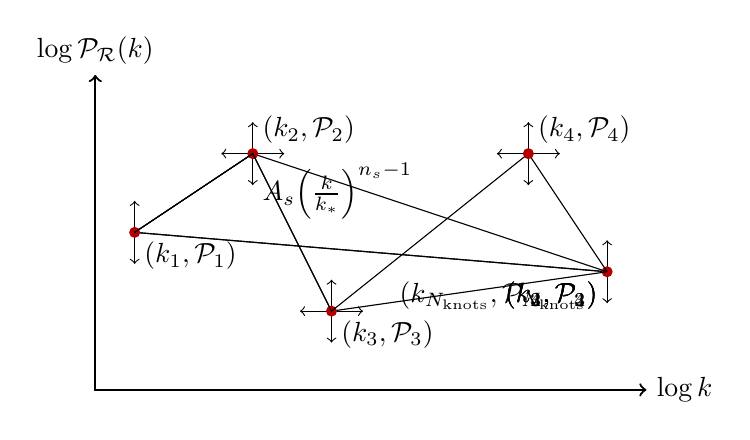
\begin{tikzpicture}
    % width of axes
      \def\xwidth{7}
      \def\ywidth{4}
    % min coordinate
      \def\xmn{0.5}
      \def\ymn{2}
    % start coordinate
      \def\xstart{2}
      \def\ystart{3}
    % middle coordinate
      \def\xmid{3}
      \def\ymid{1}
    % end coordinate
      \def\xend{5.5}
      \def\yend{3}
    % max coordinate
      \def\xmx{6.5}
      \def\ymx{1.5}

    % length of crosses
      \def\croslen{0.4}


    % Draw axes
      \draw [<->,thick] (0,\ywidth) node (yaxis) [above] {$\log\PR(k)$}
      |- (\xwidth,0) node (xaxis) [right] {$\log k$};
    % Draw limits
      %\draw [-,dashed] (\xmn,0) node[below] {$\log_{10}k_1$} -- (\xmn,\ywidth) ;
      %\draw [-,dashed] (\xmx,0) node[below] {$\log_{10}k_N$} -- (\xmx,\ywidth) ;

      \draw<1> (\xmn,\ymn) -- (\xmx,\ymx);
      \draw<1> (\xstart,\ystart) node[below right] {$A_s {\left(\frac{k}{k_*}\right)}^{n_s-1}$};

    % Draw the line joining start and end

      \coordinate (mn) at (\xmn,\ymn);
      \coordinate (start) at (\xstart,\ystart);
      \coordinate (mid) at (\xmid,\ymid);
      \coordinate (end) at (\xend,\yend);
      \coordinate (mx) at (\xmx,\ymx);
      \draw<2> (mn) -- (mx);
      \draw<2-> (mn) node[below right]    {$(k_1,\Pknotj{1})$};
      \draw<2> (mx) node[below left]     {$(k_{2},\Pknotj{{2}})$};
      \onslide<2->{\movablevert{mn}};
      \onslide<2->{\movablevert{mx}};

      \draw<3> (mn) -- (start) -- (mx);
      \onslide<3->{\movablecross{start}};
      \draw<3-> (start) node[above right] {$(k_2,\Pknotj{2})$};
      \draw<3> (mx) node[below left]     {$(k_{3},\Pknotj{{3}})$};
 
      \draw<4> (mn) -- (start) -- (mid) -- (mx);
      \onslide<4->{\movablecross{mid}};
      \draw<4-> (mid) node[below right] {$(k_3,\Pknotj{3})$};
      \draw<4> (mx) node[below left]     {$(k_{4},\Pknotj{{4}})$};

      \draw<5-> (mn) -- (start) -- (mid) -- (end) -- (mx);
      \onslide<5->{\movablecross{end}};
      \draw<5-> (end) node[above right] {$(k_4,\Pknotj{4})$};
      \draw<5-> (mx) node[below left]     {$(k_{\Nknots},\Pknotj{{\Nknots}})$};


      %\draw<2-> (\xmn,\ymn) coordinate (mn) -- (\xstart,\ystart) coordinate (start) -- (\xmid,\ymid) coordinate (mid) --  (\xend,\yend) coordinate(end) -- (\xmx,\ymx) coordinate(mx);

    % Draw the point labels
      %\draw<2-> (mn) node[below right]    {$(k_1,\Pknotj{1})$};
      %\draw<2-> (start) node[above right] {$(k_2,\Pknotj{2})$};
      %\draw<2-> (mid) node[below right]   {$(k_3,\Pknotj{3})$};
      %\draw<2-> (end) node[above right]   {$(k_4,\Pknotj{4})$};
      %\draw<2-> (mx) node[below left]     {$(k_{\Nknots},\Pknotj{{\Nknots}})$};

    % Draw a dashed line indicating the coordinate names
      %\draw[dashed] (yaxis |- start) node[left] {$y_{1}$}
      %-| (xaxis -| start) node[below] {$x_1$};
      %\draw[dashed] (yaxis |- mid) node[left] {$y_{2}$}
      %-| (xaxis -| mid) node[below] {$x_2$};
      %\draw[dashed] (yaxis |- end) node[left] {$y_{N}$}
      %-| (xaxis -| end) node[below] {$x_N$};
      %\draw  (xaxis -| start) node[below] {$\log_{10}k_2$};
      %\draw  (xaxis -| mid) node[below] {$\log_{10}k_3$};
      %\draw  (xaxis -| end) node[below] {$\log_{10}k_4$};

      % Draw the crosses
      %\onslide<2->{\movablevert{mn}
      %\movablecross{start}
      %\movablecross{mid}
      %\movablecross{end}
      %\movablevert{mx}
    %};

    % put some ellipses in between the start and end point

    \end{tikzpicture}

  }

\end{frame}


%\begin{frame}
%  \frametitle{Planck data}
%  \framesubtitle{Primordial power spectrum $\PR(k)$ reconstruction}
%  \begin{itemize}
%    \item<2-> Temperature data TT+lowP
%    \item<3-> Foreground $(14)$ \& cosmological $(4 +2*\Nknots-2)$  parameters
%    \item<4-> Marginalised plots of $\PR(k)$
%    \item<5->
%      \[ \prob(\PR|k,\Nknots) = \int \delta(\PR-f(k;\theta))\posterior(\theta)d\theta \]
%  \end{itemize}
%\end{frame}



\begin{frame}
  \frametitle<1>{0 internal knots}
  \frametitle<2>{1 internal knots}
  \frametitle<3>{2 internal knots}
  \frametitle<4>{3 internal knots}
  \frametitle<5>{4 internal knots}
  \frametitle<6>{5 internal knots}
  \frametitle<7>{6 internal knots}
  \frametitle<8>{7 internal knots}
  \frametitle<9>{8 internal knots}
  \frametitle<10>{Bayes Factors}
  \frametitle<11>{Marginalised plot}
  \framesubtitle{Primordial power spectrum $\PR(k)$ reconstruction}


  \begin{center}
    \includegraphics<1>[width=0.9\textwidth]{figures/0TT_fgivenx}
    \includegraphics<2>[width=0.9\textwidth]{figures/1TT_fgivenx}
    \includegraphics<3>[width=0.9\textwidth]{figures/2TT_fgivenx}
    \includegraphics<4>[width=0.9\textwidth]{figures/3TT_fgivenx}
    \includegraphics<5>[width=0.9\textwidth]{figures/4TT_fgivenx}
    \includegraphics<6>[width=0.9\textwidth]{figures/5TT_fgivenx}
    \includegraphics<7>[width=0.9\textwidth]{figures/6TT_fgivenx}
    \includegraphics<8>[width=0.9\textwidth]{figures/7TT_fgivenx}
    \includegraphics<9>[width=0.9\textwidth]{figures/8TT_fgivenx}
    \includegraphics<10>[width=0.9\textwidth]{figures/Bayes_TT.pdf}
    \includegraphics<11>[width=0.9\textwidth]{figures/combined_fgivenx.pdf}

  \end{center}
\end{frame}


\begin{frame}
  \frametitle{Affine invariance}
  \begin{itemize}
    \pause\item The optimal exploration technique is be affine invariant.
    \pause\item Treat distribution $\prob(\mathbf{x})$ and $\prob(R \mathbf{x})$ the same.
    \pause\item No need to worry about correlations.
    \pause\item Good example: Now highly successful emcee (MCMC hammer).
      \begin{itemize}
        \item Important: emcee is not unique (or necessarily best)
      \end{itemize}
  \end{itemize}
\end{frame}


\begin{frame}
  \frametitle{Skillings affine invariant ideas}
  \framesubtitle{Leapfrog}
\foreach \pagenum in {1,...,6} {%
  \includegraphics<\pagenum>[width=\textwidth,page=\pagenum]{figures/leapfrog}
}
\end{frame}

\begin{frame}
  \frametitle{Skillings affine invariant ideas}
  \framesubtitle{Parallel walk}
\foreach \pagenum in {1,...,6} {%
  \includegraphics<\pagenum>[width=\textwidth,page=\pagenum]{figures/parallel_walk}
}
\end{frame}

\begin{frame}
  \frametitle{Affine invariance}
  \framesubtitle{Subspace collapse}
  \begin{itemize}
    \pause\item The main problem that besets these techniques is ``subspace collapse''.
  \end{itemize}
\end{frame}

\begin{frame}
  \frametitle{Subspace collapse}
  \framesubtitle{Leapfrog}
  \includegraphics[width=\textwidth,page=6]{figures/leapfrog}
\end{frame}

\begin{frame}
  \frametitle{Subspace collapse}
  \includegraphics[width=\textwidth,page=7]{figures/parallel_walk}
\end{frame}

\begin{frame}
  \frametitle{Subspace collapse}
  \framesubtitle{Solution}
  \begin{itemize}
    \pause\item Need to use $\sim\mathcal{O}(D)$ points to avoid this.
  \end{itemize}
\end{frame}

\begin{frame}
  \frametitle{Skillings affine invariant ideas}
  \framesubtitle{Guided walk}
\foreach \pagenum in {1,...,8} {%
  \includegraphics<\pagenum>[width=\textwidth,page=\pagenum]{figures/guided_walk}
}
\end{frame}

\begin{frame}
  \frametitle{Affine invariant}
  \framesubtitle{Other variations}
  \begin{itemize}
    \pause\item Generalise guided walk to $D$ dimensions (slice through the mean of $D$ other points).
    \pause\item Slice through a ``random'' linear combination of $D$ points.
    \pause\item Slice through a ``random'' linear combination of all points
    \pause\item There are lots of variations: This is an underused area of the field.
  \end{itemize}
\end{frame}


\begin{frame}
  \frametitle{PolyChord 2.0}
  \begin{itemize}
    \pause\item Using intermediate points so $\sim\mathcal{O}(D^3)\to\sim\mathcal{O}(D^2)$.
    \pause\item Unweaving runs to quantify correlations
    \pause\item Affine invariant sampling
  \end{itemize}
\end{frame}

\end{document}
